Docker Compose ist ein Werkzeug zur Definition und Ausführung von 
Multi-Container-Anwendungen. Anstatt jeden Container einzeln manuell 
zu starten und zu konfigurieren, werden alle benötigten Services, 
Netzwerke und Volumes in einer einzigen \textbf{YAML-Datei} beschrieben 
\cite{docker_compose}.

\subsubsection{Aufbau einer Docker Compose Datei}

Eine Docker Compose Datei besteht aus drei zentralen Bereichen 
\cite{docker_compose}:

\begin{itemize}
    \item \textbf{Services}: definieren die einzelnen Container, 
    ihr Basis-Image, Umgebungsvariablen, Ports und Abhängigkeiten.
    
    \item \textbf{Networks}: definieren wie die Container miteinander 
    kommunizieren.
    
    \item \textbf{Volumes}: definieren wie Daten persistent gespeichert 
    werden, also unabhängig vom Lebenszyklus eines Containers.
\end{itemize}

Abbildung~\ref{fig:compose-example} zeigt ein einfaches Beispiel 
einer Docker Compose Datei mit zwei Services.

\begin{figure}[H]
    \centering
    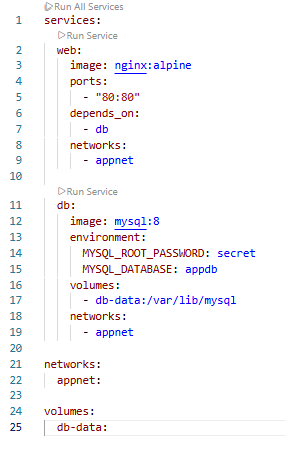
\includegraphics[width=0.75\textwidth]{pics/compose_example.png}
    \caption{Beispiel einer einfachen Docker Compose Datei}
    \label{fig:compose-example}
\end{figure}

\subsubsection{Abhängigkeiten zwischen Services}

In vielen Anwendungen müssen Services in einer bestimmten 
Reihenfolge starten. Ein typisches Beispiel: Das Backend 
versucht beim Start sofort eine Verbindung zur Datenbank 
herzustellen. Wenn die Datenbank aber noch nicht bereit ist, 
schlägt das fehl und die Anwendung startet nicht korrekt.

Docker Compose löst das mit der \texttt{depends\_on} Anweisung 
\cite{docker_compose}. Damit kann man festlegen welcher Service 
zuerst starten muss. Noch genauer wird es mit der Bedingung 
\texttt{service\_healthy}: Der abhängige Service startet erst 
dann, wenn der andere Service einen sogenannten 
\textbf{Healthcheck} bestanden hat. Ein Healthcheck ist ein 
kurzer Test der regelmäßig prüft ob ein Service wirklich 
bereit ist, also zum Beispiel ob die Datenbank tatsächlich 
Anfragen annimmt und nicht nur gestartet wurde.

\subsubsection{Netzwerke}

Standardmäßig erstellt Docker Compose für jeden Stack ein eigenes 
virtuelles Netzwerk. Alle Services innerhalb dieses Netzwerks können 
sich gegenseitig über ihren Servicenamen erreichen, ohne dass Ports 
nach außen geöffnet werden müssen \cite{docker_compose}. Das bedeutet 
zum Beispiel, dass ein Backend den Datenbankserver einfach über den 
Hostnamen \texttt{db} ansprechen kann, anstatt über eine IP-Adresse.

Zusätzlich können externe Netzwerke eingebunden werden, was besonders 
dann nützlich ist wenn mehrere Compose-Stacks miteinander kommunizieren 
sollen, etwa wenn ein Reverse-Proxy in einem eigenen Stack läuft 
\cite{docker_compose}.

\subsubsection{Vorteile von Docker Compose}

Der größte Vorteil von Docker Compose ist die \textbf{Reproduzierbarkeit}: 
Die gesamte Anwendungsinfrastruktur ist in einer einzigen Datei 
beschrieben und kann mit einem einzigen Befehl gestartet werden 
\cite{docker_compose}:

Gerade in der Teamarbeit ist das ein großer Vorteil, da alle Entwickler 
dieselbe Umgebung verwenden und Konfigurationsunterschiede zwischen 
einzelnen Rechnern ausgeschlossen werden \cite{docker_compose}.
Der gesamte Stack wird mit folgendem Befehl gestartet:

\begin{verbatim}
docker compose up -d
\end{verbatim}